\documentclass[12pt]{article}

% set margins and spacing
\addtolength{\textwidth}{1.3in}
\addtolength{\oddsidemargin}{-.65in} %left margin
\addtolength{\evensidemargin}{-.65in}
\setlength{\textheight}{9in}
\setlength{\topmargin}{-.5in}
\setlength{\headheight}{0.0in}
\setlength{\footskip}{.375in}
\renewcommand{\baselinestretch}{1.0}
\linespread{1.0}

% load miscellaneous packages
\usepackage{csquotes}
\usepackage[american]{babel}
\usepackage[usenames,dvipsnames]{color}
\usepackage{graphicx,amsbsy,amssymb, amsmath, amsthm, MnSymbol,bbding,times, verbatim,bm,pifont,pdfsync,setspace,natbib}

% enable hyperlinks and table of contents
\usepackage[pdftex,
bookmarks=true,
bookmarksnumbered=false,
pdfview=fitH,
bookmarksopen=true,hyperfootnotes=false]{hyperref}

% define environments
\newtheorem{definition}{Definition}
\newtheorem{fact}{Fact}
\newtheorem{result}{Result}
\newtheorem{proposition}{Proposition}



\begin{document}
\title{Nepobabies: Labor Market Entry and Nepotistic Behavior of Young Adults}
\author{Rachel Rabinowitz\thanks{Syracuse University, Maxwell School of Citizenship and Public Affairs. Email: rhrabino@syr.edu.} \and Ryan Seely\thanks{Syracuse University, School of Education. Email: rpseely@syr.edu. 
We would like to thank Professor Kristy Buzard and Dylan Eldred for their guidance and support. We also thank Professor Maria Zhu for her work on this project that gave us this opportunity.}}
\date{\vskip-.1in \today}
\maketitle

\vskip.2in
\begin{center} {\bf Abstract} \end{center}

\begin{quote}
{\small We examine the effects of young adults entering the workforce during competitive labor markets and whether those seeking jobs during high unemployment times will be more likely to be in their parents' occupations. We create a framework where young adults working in the same industries as their parents are defined as products of nepotism and examine how such products of nepotism find employment under varying economic conditions. Our analysis uses two-sample t-tests and chi-square analysis to examine the differences in rates of nepotism for varying levels of unemployment. Using data on young adults hired between 1960 and 2022, we find a greater likelihood of gaining employment within the same industry as ones parents during poor economic conditions with high unemployment. }
\end{quote}


\bigskip
\section{Introduction} \label{sec:introduction}
"Nepobaby" is a term commonly used to describe nepotism among families, specifically among children of celebrities. The term is mostly used as an insulting phrase to imply someone's success was unearned and undeserving as they have had disproportionate access to the labor market through their connections. This popular term, which is now used to encompass the general population, extends to those receiving employment or other benefits through familial connections in industries. Within our study, we define nepobabies as respondents who work in the same industry as at least one of their parents.

Our study examines whether nepobabies are more likely to be hired in competitive labor markets. By matching monthly employment rates to the estimated month in which someone was hired, we examine the relationship between the level of labor market competition and the likelihood of having a nepotistic industry relationship with a parent.
During times of competitive labor market conditions, young adults attempting to enter the workforce experience many difficulties. These young adults struggling to enter into the workforce may turn to their connections to seek employment. As young professionals gain employment through relatives, nepobabies appear in the overall working population. This struggle for young professionals will incentivize them to use all of their resources to find a job. Therefore, we predict that there will be more graduates joining their parent’s occupations under these conditions. 


Using data from the General Social Survey (GSS) and the Federal Reserve Economic Data (FRED), we analyze the relationship between labor market conditions and prevalency of nepobabies. Through two-sample t-tests, we gather enough evidence to reject our null hypothesis that there is no relationship between nepotism rates and the level of labor market competition. Nepobabies were found to have been hired during higher unemployment times at a significantly greater rate than during less challenging economic times. Dividing our sample into  quartiles based on unemployment rates, we find a notable discrepancy between the rates of nepobabies hired in low versus high unemployment. Through further two-sample t-tests, nepobabies were also found to follow the same profession as their gendered parent. Daughters were more likely to follow into their mother's profession and sons were more likely to follow into their father's. Through further testing on other characteristics in our sample, nepobabies feel greater job security within their workplaces.


\section{Literature Review} \label{sec:literature}
In recent decades, there have been many studies on relationships between parents and their children, the outlook of entering the workforce in tough economics times, and using social ties to gain employment. Specifically within the workforce, the effects of graduating college during competitive labor markets have been largely analyzed. Khan (2010) describes the relationship between graduating in tough economic conditions and one's ability to find employment within the first two decades after graduation. By graduating in a worse-off economy, recent graduates should be expected to experience higher unemployment resulting in a greater likelihood of job mismatching. Job mismatching, a situation in which workers are forced into specific jobs that do not correspond with their education level or qualifications have resulted in many being pushed to seek higher education, hoping to both increase their human capital and to enter the workforce during better economic times. Schwandt and Von Wachter (2019) and Oreopoulos, Von Wachter, and Heisz (2012) describe the increasing likelihood to seek higher education during recessions or poor economic periods. The fewer jobs demanded in a competitive labor market will be more favorable to higher-skilled workers, impacting the ability for recent graduates to find work after graduation. As a result, recent graduates entering the workforce may feel compelled to increase their human capital. The ability to differentiate oneself after graduation is a helpful tool in order to gain employment, especially in tight labor markets. This process of distinguishing oneself, attained through higher education, results in those more likely to move quickly throughout firms as they are in higher-demand than others. These highly-skilled individuals  may also be increasingly more likely to seek employment within lower-skilled jobs as they have much more variation within firms. 

Specifically within family units, Kramarz and Skans (2014) discuss how important strong family ties are when seeking stable employment. As employees are more likely to disseminate information about job openings to their strong ties first due to stable networks and greater maintenance, those having close relationships with high-skilled individuals hear about job openings first. Firms also have become increasingly dependent on recruiting from social ties. The social connections of high-quality incumbent workers have become increasingly popular as firms believe these connections will exhibit the same qualities, especially when ex-ante information about the applicant is poor. Additionally, as described by both Kramarz and Skans (2014) and Hellerstein and Morril (2011), firms benefit from recruiting children of incumbent employees. Within recent decades, young females have become increasingly more likely to enter the same profession as their fathers. Daughters may feel as if they have some sense of inside knowledge and/or networking, convincing those to feel compelled to follow into the same profession, especially during tough economic times. Women, who are described as risk-adverse by Hellerstein and Morril (2011) may follow into their parents professions, specifically their father’s occupation to prevent the risk of being jobless after their graduation. 

Few studies discuss both the impact of graduating within competitive labor markets and the likelihood of using parents as social ties to gain employment. As discussed in previous economic literature, young adult children rely deeply on their relationships to gain employment, but few discuss the relationship between children’s reliance on their ties during poor economic conditions.


\section{Data}
\label{sec:data}
We use data collected from the GSS in the years 2002, 2006, 2010, 2014, 2018, and 2022. The surveys are largely conducted through 90-minute in-person interviews with English and Spanish-speaking adults to create a nationally representative sample. Only observations from the aforementioned years were analyzed due to a key variable (job length), which measures the approximate number of years a respondent has occupied their current job, being present in these six survey years. Using this variable, we estimated the month in which a respondent was hired. Using the respondent’s age and estimated job length, we were able to limit our sample to those hired as young adults, which we defined as younger than 30 years old. After limiting our sample to young adults and the years where the job length variable was present, there were 3,550 (3,550 figure must be checked again, something that Prof. Buzard noted) observations of young adults and 287 young adult nepobabies. We defined nepobabies as having a matching industry code with at least one parent based on the 2007 North American Industry Classification System (NAICS) codes. 

The GSS data set, however, does not include data on unemployment rates at the time a respondent was interviewed or hired. Therefore, we used a monthly unemployment rate data set from the Federal Reserve Economic Data (FRED). Using the FRED data merged with the GSS data set, we were able to assign an unemployment rate for the estimated month at which a respondent was hired. The monthly unemployment rate data spanned every month from January of 1960 to December of 2022 to include the range of all possible months a respondent in our data set was hired. 


\section{Results}
\label{sec:result}

In the first part of our analysis, we attempt to show how nepotistic behavior changes when labor markets become more competitive. In the second part, we analyze the demographics and parental relationships of nepobabies.


We created four groups of nepobabies, hired during low unemployment, hired during mid-low unemployment, hired during mid-high unemployment, and hired during high unemployment. In our analysis, low unemployment is considered to be an unemployment rate of less than or equal to 4.5 percent. Mid-low unemployment is considered to be greater than 4.5 percent but less than or equal to 5.4 percent. Mid-high unemployment is considered to be between 5.4 percent and 6.7 percent unemployment. High unemployment is considered to be greater than 6.7 percent. We determined these to be the cutoff for high and low unemployment rates because they represent the values marking each of the quartiles of all unemployment rates in our sample of hire months. By creating these four groups based on the quartiles, we create groups that are of roughly equal sizes of all respondents and optimal for performing two-sample t-tests that compare the difference between the number of nepobabies in each group, as shown in the table below.

\begin{table}[ht]
\centering
\begin{tabular}{l|cc|c}
Hire Group & Nepobabies & Non-Nepobabies & Proportion \\ 
\hline 
Low & 53 & 899 & 0.059 \\
Mid-low & 75 & 839 & 0.089\\
Mid-high & 75 & 704 & 0.107 \\
High & 84 & 821 & 0.102 \\
\hline 
Sample & 287 & 3,263 & 0.088 \\
\end{tabular}
\caption{Unemployment Level Hire Group Frequency Table}
\label{tab:mytable}
\end{table}



We decided to measure the difference in means between the quartiles to find any statistical significance between the number of nepobabies in each unemployment level hire group. If there is a statistically significant difference between the number of nepobabies in each group as we have defined them, then that provides evidence for our hypothesis that a greater level of labor market competition will produce a greater amount of nepotism hires. It is important to note here that we cannot determine the actual level of nepotism per se, rather it is more a reflection of the level of young adults joining the same industry as their parents. However, it is safe to assume that there is a positive association between the two levels.


After categorizing our sample of nepobabies in this manner, we conducted mutilple two-sample t-tests measuring the statistical significance of the means between nepobabies hired in varying levels of employment. Our null hypothesis is that there was no significant difference between the mean of nepobabies hired during higher unemployment times and the mean of nepobabies hired during lower unemployment times. First we tested the difference between the highest unemployment rate group (unemployment greater than or equal to 6.7 percent) and the lowest unemployment rate group (unemployment less than or equal to 4.5 percent). With 99 percent confidence, we can say that the number of nepobabies hired during high unemployment is significantly greater than the number of nepobabies hired during low unemployment. This first result provides strong evidence for our hypothesis that during competitive labor markets, young adults have greater incentive to use all of their resources to find a job, with a main resource being their parents.  We then tested the relationships between mid-low (unemployment greater than 4.5 and less than or equal to 5.4 percent) and mid-high (unemployment greater than 5.4 and less than 6.7 percent) unemployment level groups with the others. From the two-sample t-test between the mid-low and low unemployment level groups, the result is, at a 95 percent confidence level, that there are significantly more nepo-babies hired during the mid-low unemployment level. This provides further evidence that young adults are more likely to use their resources to find employment when the labor market is more competitive. The final two t-tests we ran provide evidence for the hypothesis, but add a new dimension to our analysis that warrants further study. The number of nepobabies hired during the mid-low and mid-high level unemployment levels are the same; 75. This can be seen in Table 1 and the two-sample t-test for this comparison provides the same result. The last two-sample t-test ran compares the number of nepobabies hired between the high unemployment and mid-high unemployment groups.  We find that there is no statistically significant difference between the number of nepobabies in those two groups. This means that the number of nepobabies hired in high unemployment, mid-high unemployment, and mid-low unemployment, are roughly the same. The dimension that this adds is that relying on nepotistic relationships with parents to find unemployment may be typical behavior that holds for most unemployment levels, except when the labor market is particularly noncompetitive, in which case young adults do not feel the need to rely on their parents for support. We show the difference in the number of nepobabies hired during different unemployment levels in Figure 1 above. 

\begin{figure}
    \centering
    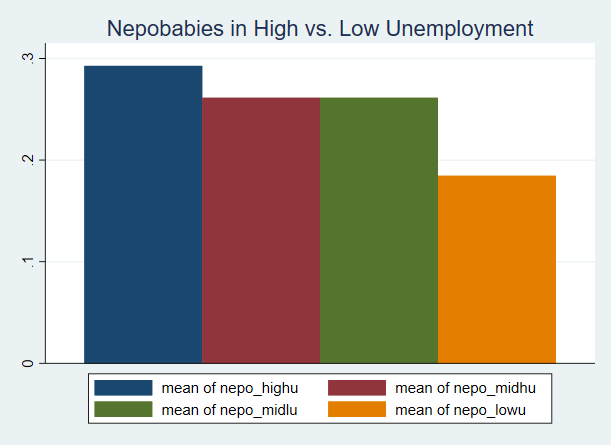
\includegraphics[width=0.65\linewidth]{nepobabies_percentile_categories.pdf}
    \caption{Frequency of Nepobabies Hired at Varying Labor Market Conditions}
    \label{fig:enter-label}
\end{figure}


\begin{table}[ht]
\centering
\begin{tabular}{c|cccc|c}
  & \multicolumn{4}{c}{Unemployment Level} &   \\
Nepotism Status & Low & Mid-Low & Mid-high & High   & Total \\
\hline
Nepobaby & 53 & 75 & 75 & 84 & 287 \\
Non-nepobaby & 899 & 839 & 704 & 821 & 3,263 \\
\hline
Total & 952 & 914 & 779 & 905 & 3,550 \\
\end{tabular}
\caption{Nepotism Status and Unemployment Level Hire Group Frequency Table}
\label{tab:mytable}
\end{table}


The analysis above using the two-sample t-tests looks exclusively at the frequency of nepobabies hired under different labor market competition levels and it does not account for the amount of non-nepobabies hired under the same competition levels. To include this important component into our analysis, we compare the ratios of nepobabies to non-nepobabies hired at the different unemployment levels and then perform a chi-squared test. In the Table 2, the importance of considering the ratio of nepobabies to non-nepobabies hired at the different unemployment levels can be seen. Whereas in Figure 1 the number of nepobabies hired at the mid-low and mid-high unemployment levels were equal, in Table 2 the difference between the ratio of those hired at those levels can be seen. In order to evaluate the significance of these ratios, we performed a chi-squared test in order to determine if the difference in the ratios is due to chance or if there is something else at play, as our hypothesis suggests.




The results of the chi-squared test are strong and suggest that our research hypothesis has great merit. With three degrees of freedom and at a 99 percent confidence level, there is enough evidence to reject the null hypothesis of this test, that there is no association between unemployment level and nepotism status. In figure two, the ratios of nepobabies to non-nepobabies hired at varying levels are shown and compared to one another. It is clear that hiring under greater labor market competition has an association with the rate of nepotistic behavior. This conflicts with the aforementioned suggestion that nepotistic behavior is the standard and low rates of labor market competition lessens the reliance on it. The ratios displayed in Figure 2 suggest that above average labor market competition compels young adults to utilize the resource that is their parents to find employment, and that below average competition does not drive young adults to utilize that resource at the same rate.


\begin{figure}
    \centering
    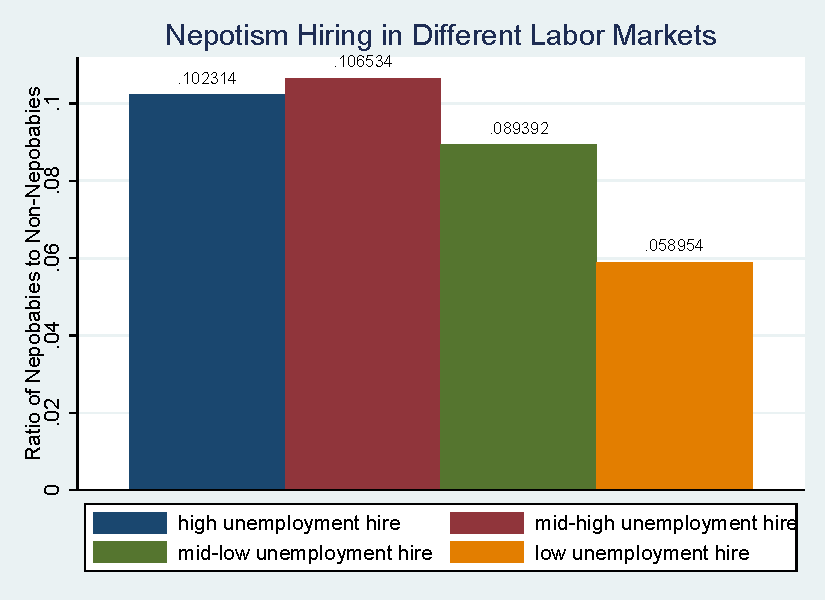
\includegraphics[width=0.65\linewidth]{NepoHireRatioBarGraph.pdf}
    \caption{Ratios of Nepotism Hiring}
    \label{fig:enter-label}
\end{figure}

For the second part of our analysis, we looked at the gender dynamics of nepotistic parent-child relationships and the demographics of nepobabies. As expected, we find that children are much more likely to find themselves in a nepotistic relationship with their parent of the same gender than they are for the opposite gender parent. Nepotistic mothers, of which there were 118 when excluding mothers who had the same industry as the respondent’s father, were much more likely to have their daughters in the same industry than their sons. Of the nepotistic mother-child relationships, 71 percent were daughters and only 29 percent were sons. This highly gendered relationship holds true for nepotistic fathers. When excluding fathers who had the same industry as the respondent’s mother, there were 145 nepotistic fathers. Of the nepotistic father-child relationships, 80 percent were sons and only 20 percent were daughters. 


We then examined different demographics, as recorded in the GSS observations, to compare nepobabies to the rest of the sample. First, we tested how race differs between the sample and the nepobaby population within our sample. The sample is 72.3 percent white and the nepobabies are 77.4 percent white. After running a two-sample t-test to measure the significance of the difference of means between these two populations, we find that the difference is statistically significant, and can say with 95 percent confidence that nepobabies are more likely to be white than their counterparts whose parents are in different industries. We ran similar chi-square analysis and found no statistically significant association between nepobaby status and the following demographics: gender, income, and class (self-reported).

We also examined how nepobabies may behave differently in the workplace than their counterparts. Using a variable that marks the likelihood that a respondent thinks they will lose their job, we found that nepobabies feel more secure in their workplaces. While only 65 percent of all workers in our sample said they think it is not likely that they will lose their job, 73 percent of nepobabies believe that it is unlikely they will lose their job. From the two-sample t-test we ran, we can say with 95 percent confidence that there is a statistically significant difference between the proportion of nepobabies who feel more confident in the safety of their employment status than the rest of the sample. This provides further evidence of the benefit that nepobabies receive by taking advantage of their parental connections to find and maintain employment. We found no statistically significant difference between nepobabies and the entire sample in terms of another work related feature in the data set, hours worked per week. From the two-sample t-tests we ran, nepobabies were not more or less likely to work overtime or part-time.

From the statistical tests we performed, we have confidence that there is a positive association between the level of unemployment (representing the competitiveness of the labor market) and the rate of nepotism among young adults joining the labor market. Our hypothesis that we sought to test is that when labor markets are more competitive, young adults will be compelled to take advantage of their resources, specifically their parents, and create nepotistic relationships in order to find employment. From the multiple two-sample t-tests and the chi-squared analysis, we have enough evidence to reject the null hypothesis, that the level of labor market competition does not drive differences in the rate of nepotistic relationships between young adults and their parents. We also find that nepobabies are more likely to be white and are more likely to feel safe in their job, providing us with some information on who nepobabies are and how being a product of nepotism has altered their working experience.

 



\section{Discussion}
\label{sec:discussion}
The results from our analysis provide strong evidence for our hypothesis, however there are additional analyses and factors that limit the strength of our results and give opportunity for others to build on our findings. First, there are some limitations in our data 
sets that could be addressed in future research. The FRED unemployment rate data set that we used to evaluate were national averages of the U.S. unemployment rate. Of course, that average does not necessarily pertain to each observation/individual. Future work could use state averages to better estimate the effects of labor market competition on rates of nepotism. Additionally, the variable we used to estimate the month at which a GSS respondent was hired was not perfectly accurate. Respondents could only answer that they had been employed at their current job for three months, nine months, or whole years starting at 1 and counting up. This means that the month of hire we assigned for each respondent may not be exact. More precise measures of the amount of time someone has held their job could allow for more accurate analysis. Lastly, we would like to expound on the limitations of how nepobaby is defined. We defined nepobabies as having at least one parent in the same industry as the respondent, with the industry matching based on the 2007 North American Industry Classification System (NAICS) codes. However, just because someone is in the same industry as a parent does not mean that they were on the receiving end of nepotism in finding employment. Additionally, just because someone is not in the same industry as one of their parents does not mean that they were not on the receiving end of nepotism. For example, a young adult may have used other resources like extended family and friends to create nepotistic relationships to find employment, likely demonstrating that they went to further lengths to find employment. Our data set does not contain information on this type of nepotism or on the amount of effort a person put into using their resources for finding employment. Additional analysis would benefit from obtaining information on these other forms of nepotism and on how respondents used their resources to gain employment so that this could be analyzed over the business cycle.


We also encourage policymakers and administrators in secondary and higher education to examine these results and consider their implications. While we only found a few areas where nepobabies had significantly different characteristics than the sample at large, this analysis was limited by the characteristics noted in the GSS data set. However, it can be certain that such nepotistic relationships and their support in helping young adults find jobs gives an advantage to those who have living, working parents and to those who have good relationships with their parents. The use of such nepotistic relationships inherently creates an inequality between young adults who can use their parents’ status to gain employment and young adults who do not have that resource. Policymakers and administrators of educational institutions, especially those focused on creating equity, may find these results troubling. Support systems for those who cannot access these resources may be put into place to give those who lack such resources an equal opportunity to find employment, especially students of color who were significantly less likely to have gained employment through a nepotistic relationship with a parent.


\section{Conclusion}
\label{sec:conclusion}

Labor market competition levels significantly impact the ability of graduates to find employment after graduation. Nepotistic relationships, where a young adult works within the same industries as at least one of their parents, have a greater likelihood of forming during poor economic times. By matching respondents’ industries to their parents’ professions, the respondents classified as nepobabies were seen in higher numbers during times with high unemployment rates. We provide evidence for the theory that under times of competitive labor markets, labor market entrants will be more inclined to use their resources to find stable employment, relying on their parents. 
We use two data sets, both pertaining to data within the United States. The GSS offers data on respondents' answers to questions including their demographic information, employment status, and questions regarding family relationships. The FRED data set includes monthly unemployment rates from 1960 to 2022. These data sets allow for a preliminary evaluation of young adults, specifically those in nepotistic relationships, gaining employment during different economic conditions.
Measuring the times in which someone was hired and matching this time to the monthly unemployment rate indicates if nepotism was used under more competitive labor market conditions. As noted in the literature review, poor economic conditions result in labor market entrants experiencing difficulty entering the workforce. By gaining employment through relatives, specifically parents, young professionals create nepotistic relationships as a form of using resources to find employment. Through economic cycles, nepobabies are more commonly found in times of higher unemployment. Young adults experiencing competitive labor market conditions upon entering the labor market are met with greater obstacles, pushing some to follow into their parent's profession and ultimately to become nepobaby. 



\newpage
\section*{Bibliography}
\singlespacing
\setlength\bibsep{1pt}

\hspace{1cm}Hellerstein, J. K., and Morrill, M. S. (2011). Dads and Daughters: The Changing Impact of Fathers on Women’s Occupational Choices. The Journal of Human Resources, 46(2), 333–372. http://www.jstor.org/stable/41304823

Kahn, L. B. (2010). The long-term labor market consequences of graduating from college in a bad economy. Labour economics, 17(2), 303-316.

Kramarz, F., and Skans, O. N. (2014). When strong ties are strong: Networks and youth labour market entry. Review of Economic Studies, 81(3), 1164-1200.  



Oreopoulos, P., Von Wachter, T., and Heisz, A. (2012). The short- and long-term career effects of  graduating in a recession. American Economic Journal: Applied Economics, 4(1), 1-29.


Schwandt, H., and Von Wachter, T. (2019). Unlucky cohorts: Estimating the long-term effects of entering the labor market in a recession in large cross-sectional data sets. Journal of Labor Economics, 37(S1), S161-S198.


\end{document}
